\fancychapter{Analysis}
Explain the timeline of the work done on this project. When reading this section, the reader will understand how all the chapters of this thesis fit together. 
Its like a introduction where the next four chapters are interconnected.

\fancychapter{Clustering Tweets with Self-Organizing Maps}
Work done on the INESC twitter dataset with SOMs.
SOM implementations used, what where their strong points and weaknesses
SVM Dimension reduction and text treatment: compare multiple aproaches to reduce the svm size of tweets without losing relevant information

\fancychapter{Crawling Twitter for Social Relations}
Explain the limitations of the INESC tweet dataset: crawlled by hashtag, social connections can only be obtained through connections to the twitter API, a lot of the tweets had no active users etc. 

\fancychapter{SOM Framework}
Explain what got me to create my own ruby library: everybody is making their own SOM algorithms ( ex.: websom, hsom etc ). Most implementations want to get as close to the metal as possible in order to deliver faster trainings, which makes the lybraries hard to modify. SOM framework is an modular implementation of the SOM algorithm in an higher level programing language which makes it easier to construct and test new SOM algorithms.

\fancychapter{Homophilic SOM}
Describe the alterations made to the default SOM algorithm in order to increase the homophilic (love of the same) relevance while cathegorizing socially connected data.

%% Sub multiple figures
%
%\begin{figure}[t]
%\centering
%\subfigure[caption for subfigure a]{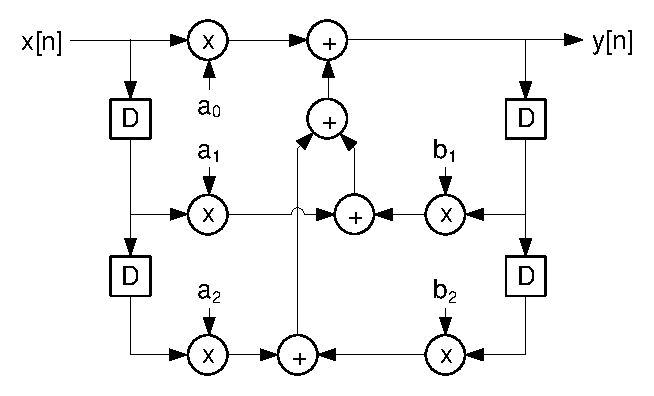
\includegraphics[scale=0.65]{images/img1.eps}\label{chp3:img1}}
%\hspace*{0.5cm}
%\subfigure[caption for subfigure b]{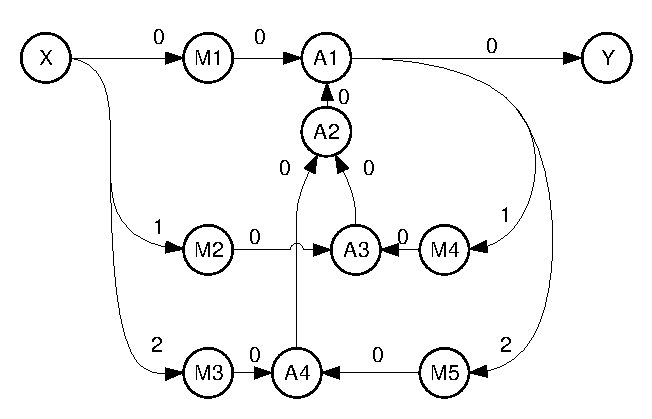
\includegraphics[scale=0.65]{images/img2.eps}\label{chp3:img2}}\\
%\caption{A figure example.}
%\label{fig:rmain figure}
%\end{figure}
%See the source code to see how to reference each of the subfigures \ref{chp3:img1} or \ref{chp3:img2}, or the main figure \ref{fig:rmain figure}.

%% how to add formulas
%There are several ways to define formulas (see the \textit{Short Math Guide for LaTeX} included in the package). The typical method is to use (see source code): 
%\begin{equation}
%a= b + c
%\end{equation}
%or
%\begin{align}
%c &= d \cdot e \nonumber\\
%d &= \mathbf{X}^{\mathsf{T}} \mathbf{Y}+ \gamma e^{2\pi}
%\label{chp3:eq1} 
%\end{align}
%or
%\begin{subequations}
%\begin{align}
%c &= d \cdot e \label{chp3:eq2:a} \\
%d &= \mathbf{X}^{\mathsf{T}} \mathbf{Y} + \gamma e^{2\pi}
%\label{chp3:eq2:b} 
%\end{align}
%\label{chp3:eq2} 
%\end{subequations}
%where $\mathbf{X}$ and $\mathbf{Y}$ are column vectors (you should always present the meaning of each parameter). The \textbf{AMS} packages allow to use the command \verb"\eqref" to cite equations such as \eqref{chp3:eq1},  \eqref{chp3:eq2:a},\eqref{chp3:eq2:b} or \eqref{chp3:eq2} (see source code).


% Ensure that the next chapter starts in a odd page
\cleardoublepage
 
